% !TeX root = main.tex
\section{Note on Custom Implementation}
\label{sec:note-custom-impl}

The given \texttt{starter\_code.ipynb} (mirrored in \texttt{src/starter\_code.py}) was not used and a custom implementation was done in the \texttt{src} folder. This was done because

\begin{itemize}
    \item The custom implementation uses \href{https://docs.sympy.org/latest/index.html}{sympy} under-the-hood to handle integration and solving constraints. This makes using Wolfram Alpha not necessary.
    \item The custom implementation can scale better for different values of $n$. Only some changes in the number of constraints in the source code will be required (only two places), rest everything will scale accordingly. The starter code provided will have to be entirely re-written for different $n$ values.
\end{itemize}

To see that they both give the same results, the script \texttt{comp\_starter\_custom.py} can be used. It shows the matching results and images (visualizing trajectories with the same constraints).

\begin{figure}[ht]
    \centering
    \begin{subfigure}[b]{0.6\textwidth}
        \centering
        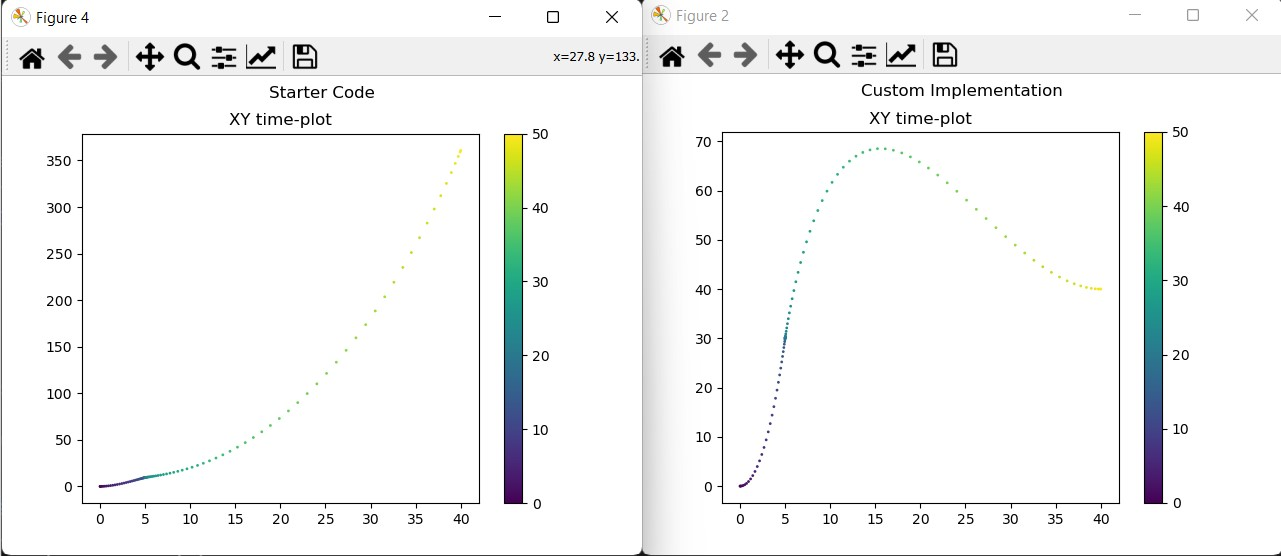
\includegraphics[width=\textwidth]{xy-comp.jpg}
        \caption{XY plot}
    \end{subfigure}
    \begin{subfigure}[b]{0.3\textwidth}
        \centering
        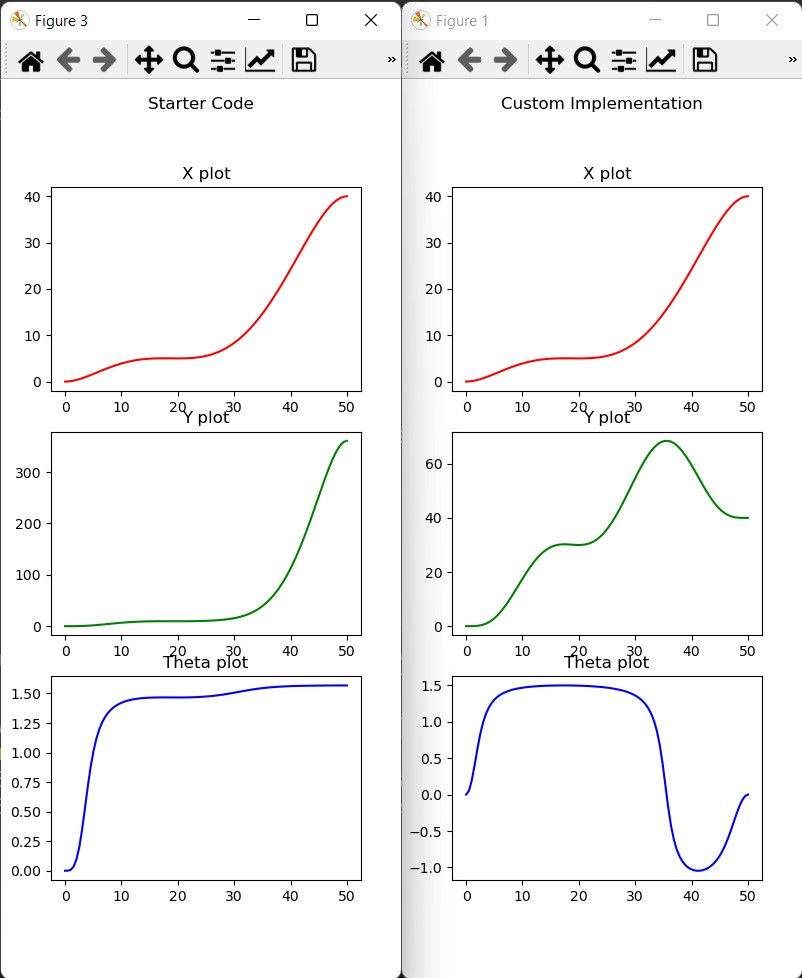
\includegraphics[width=\textwidth]{xyth-comp.jpg}
        \caption{X, Y, $\theta$ plot}
    \end{subfigure}
    \caption{Comparison of custom and starter codes}
    \label{fig:custom-starter-traj-comp}
    \small
        For each of the image above, the left window is starter code and the right one is the custom implementation.
\end{figure}

As we can see in figure \ref{fig:custom-starter-traj-comp}, the starter code fails in some cases, specially when the angle $\theta \approx 90^\circ$ (which is when $\tan(\theta) \rightarrow \infty$). The custom implementation, resolving the set of equations (and not being hard-coded), can recover (up to a limited extent).

\paragraph{Additional Notes} for practicality of the submission

\begin{itemize}
    \item The angle constraint at waypoint was dropped (both the $k$ and $\dot{k}$ constraints are not applied). This was done to get a stable Bezier curve. 
    \\
    Usually these things are deployed over small stretches and linked using terminal constraints. It is impractical to fit one through the entire path. This is \emph{smooth patching} of multiple Bezier curves.
\end{itemize}

The main submission starts from the next section.
